
\documentclass{beamer}




\mode<presentation>
{
  \usetheme{Warsaw}
  % or ...

  \setbeamercovered{transparent}
  % or whatever (possibly just delete it)
\useoutertheme{infolines}
}


\usepackage[english]{babel}
% or whatever

\usepackage[utf8]{inputenc}
% or whatever

\usepackage{times}
\usepackage[T1]{fontenc}



\title[Diferencirana zasebnost] 
{Splošna definicija diferencirane zasebnosti}


\author[Metod Jazbec] 
{Metod Jazbec
\newline
\newline
Mentor: prof. dr. Aljoša Peperko}


\institute[FMF] 
{
  
  Fakulteta za matematiko in fiziko\\
  Univerza v Ljubljani
 }


\date[DS 2018] % (optional, should be abbreviation of conference name)
{Diplomski seminar, 2018}
% - Either use conference name or its abbreviation.
% - Not really informative to the audience, more for people (including
%   yourself) who are reading the slides online





% If you have a file called "university-logo-filename.xxx", where xxx
% is a graphic format that can be processed by latex or pdflatex,
% resp., then you can add a logo as follows:

% \pgfdeclareimage[height=0.5cm]{university-logo}{university-logo-filename}
% \logo{\pgfuseimage{university-logo}}



% Delete this, if you do not want the table of contents to pop up at
% the beginning of each subsection:
%\AtBeginSubsection[]
%{
%  \begin{frame}<beamer>{Kazalo vsebine}
%    \tableofcontents[currentsection,currentsubsection]
%  \end{frame}
%}


% If you wish to uncover everything in a step-wise fashion, uncomment
% the following command: 

%\beamerdefaultoverlayspecification{<+->}

\setbeamertemplate{caption}[numbered]
\begin{document}

\begin{frame}
  \titlepage
\end{frame}

\begin{frame}[allowframebreaks]{Kazalo vsebine}
  \tableofcontents
  % You might wish to add the option [pausesections]
\end{frame}


% Structuring a talk is a difficult task and the following structure
% may not be suitable. Here are some rules that apply for this
% solution: 

% - Exactly two or three sections (other than the summary).
% - At *most* three subsections per section.
% - Talk about 30s to 2min per frame. So there should be between about
%   15 and 30 frames, all told.

% - A conference audience is likely to know very little of what you
%   are going to talk about. So *simplify*!
% - In a 20min talk, getting the main ideas across is hard
%   enough. Leave out details, even if it means being less precise than
%   you think necessary.
% - If you omit details that are vital to the proof/implementation,
%   just say so once. Everybody will be happy with that.

\section{Uvod - opis teme}


\begin{frame}{Uvod - opis teme}
  % - A title should summarize the slide in an understandable fashion
  %   for anyone how does not follow everything on the slide itself.

  \begin{itemize}
  \item Doba podatkov. Kako podatke primerno zaščititi?
  \item Veliko neprimernih metod, potreba po strogi matematični definiciji zasebnosti.
\item Diferencirana zasebnost, lepa teorija a neuporabna v praksi?
 \item Objavljanje in rudarjenje podatkov.
  \end{itemize}
\end{frame}

\begin{frame}{Uvod - opis teme}
  % - A title should summarize the slide in an understandable fashion
  %   for anyone how does not follow everything on the slide itself.

  \begin{itemize}
  \item 'American Health Care Records' primer.
  \end{itemize}
\begin{figure}
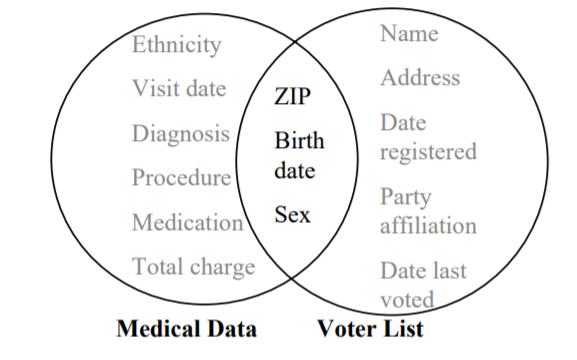
\includegraphics[width=\textwidth,height=0.5\textheight,keepaspectratio]{slika1}
\caption{Metoda anonimizacije in napad s pomožno podatkovno bazo.}
\end{figure}

\end{frame}

\begin{frame}{Uvod - opis teme}
\begin{table}
\begin{center}
 \begin{tabular}{| c | c |} 
 \hline
 \textbf{Pacient} & \textbf{Diabetes}  \\ [0.5ex] 
 \hline
 Anja & 1  \\ 
 \hline
 Bojan & 1\\
 \hline
 Cene & 0 \\
 \hline
 Darja & 0  \\
 \hline
 Edi & 1  \\  
 \hline
\end{tabular}
\caption{Podatkovna baza z imeni pacientov in podatki o diabetesu.}
\end{center}
\end{table}
  \begin{itemize}
  \item Apple primer ('data mining').
 \item \textbf{Tema diplomskega dela:} splošen model zasebnosti, ki omogoča enotno obravnavo različnih vrst podatkov.
  \end{itemize}
\end{frame}


\section{Matematična priprava}

\subsection{Monotoni razredi}

\begin{frame}{Monotoni razredi}
\begin{block}{Definicija (Monoton razred)}
Monoton razred $\mathcal{M}$ je družina podmnožic $\Omega$ (torej $\mathcal{M} \subset \mathcal{P(\mathcal{M})}$) z naslednjima lastnostima:
\begin{itemize}
\item  $\{A_i\}_{i=1,...\infty} \in \mathcal{M}, A_i \subseteq A_{i+1} \Rightarrow \bigcup_{i=1,...\infty} A_i \in \mathcal{M}$ (zaprtost za monotono naraščajoče števne unije),
\item  $\{A_i\}_{i=1,...\infty} \in \mathcal{M}, A_i \supseteq A_{i+1} \Rightarrow \bigcap_{i=1,...\infty} A_i \in \mathcal{M}$ (zaprtost za monotono padajoče števne preseke).
\end{itemize}
\end{block}
\begin{itemize}
\item Vsaka $\sigma$-algebra je monoton razred.
\end{itemize}
\end{frame}

\begin{frame}{Monotoni razred}
\begin{itemize}
\item Karakterizacija $\sigma(\mathcal{S})$ kot najmanjši monoton razred, ki vsebuje algebro $\mathcal{S}$.
\end{itemize}
\begin{block}{Izrek (O monotonih razredih)}
Naj bo $\mathcal{S}$ algebra in $\mathcal{M}$ monoton razred na množici $\Omega$. Naj velja še $\mathcal{S} \subseteq \mathcal{M}$. Potem sledi $\sigma{(\mathcal{S})} \subseteq \mathcal{M}$.
\end{block}
\end{frame}

\subsection{Kompaktnost metričnih prostorov}

\begin{frame}{Osnovno o metričnih prostorih}
\begin{block}{Definicija (Kompaktnost metričnih prostorov)} 
Metrični prostor $(D, \rho)$ je \textit{kompakten}, če ima vsako zaporedje v $D$ konvergetno podzaporedje z limito prav tako v $D$ (povedano drugače, vsako zaporedje v $D$ ima vsaj eno stekališče vsebovano v $D$).
\end{block}
\begin{itemize}
\item Ni najbolj splošna definicija kompaktnosti.
\item  $a, b \in D^n$, $\rho_H(a,b) :=$ \# mest, na katerih se vektorja razlikujeta (Hammingova razdalja/metrika)
\item $D$ kompakten, $diam(D) := \max\limits_{d,d' \in D}\rho(d,d')$
\end{itemize}
\end{frame}


\section{Splošni podatkovni model}

\subsection{Podatkovna baza}
\begin{frame}{Splošni podatkovni model}
$(U, \rho)$ poljuben metrični prostor in $D \subseteq U$. Posamezni vnosi v opazovani podatkovni bazi so elementi množice $D$. Celotno bazo prikažemo z vektorjem \textbf{d} $= (d_{1}, ..., d_{n}) \in D^n$, kjer $d_{i} \in D$ predstavlja i-ti vnos oz. vrstico.
\newline
\newline
\begin{itemize}
\item Množico $U$ opremimo z Borelovo $\sigma$ -algebro, označimo jo z $\mathcal{A}_{U}$. 
\end{itemize}
\end{frame}


\begin{frame}{Primeri različnih vrst podatkov}
\begin{itemize}
\item \textbf{Kategorični podatki:} množica hobijev, $\mathcal{H}=\{nogomet, kitara,...\}$, $D = 2^\mathcal{H}$, diskretna metrika
\item \textbf{Numerični podatki:} RGB slike dimenzije $n \times m$, $D = \mathbb{R}^{n\times m \times 3}$, $\rho(A,B)=\sum_{i,j,k}  |a_{i,j,k}-b_{i,j,k}|$,  $\mathcal{A}_{D}=\{A_{1} \times A_{2} \times A_{3} | A_{1} \in \mathcal{B}(\mathbb{R}^n),  A_{2} \in \mathcal{B}(\mathbb{R}^m),  A_{3} \in \mathcal{B}(\mathbb{R}^3) \}$
\end{itemize}
\end{frame}

\begin{frame}{Primeri različnih vrst podatkov}
\begin{itemize}
\item \textbf{'Mešani' podatki:} zdravstevni podatki, $D=\{1,2,...,st. pacientov\} \times \{1,...,120\} \times \{M,Z\} \times 
\{Ljubljana, ...\} \times \{0,1\}^n$, $\rho$ in $\sigma$-algebra podobno kot zgoraj (one-hot encoding)
\item \textbf{Funkcijski podatki:} merjenje porabe elektrike,  $D = l_{\infty}$ ali $D = L_2([0,T])$, Banachovi prostori
\end{itemize}
\end{frame}

\begin{frame}{Sosednje podatkovne baze}
Pravimo da sta dve podatkovni bazi, \textbf{d}$= (a_{1},...,a_{n})$ in $\textbf{d'}= (b_{1},...,b_{n})$,  \textit{sosednji}, če se razlikujeta v natanko enem vnosu. Torej:
\begin{itemize}
\item obstaja $j\in\{1,...n\}$, da velja $a_{j} \neq b_{j}$,
\item za vsak $i\in\{1,...,n\} \setminus j$ velja $a_{i} = b_{i}$.
\end{itemize}
Sosednji bazi označimo z \textbf{d} $\sim$ \textbf{d\'}.
\end{frame}

\subsection{Poizvedba (query)}

\begin{frame}{Poizvedba}
\begin{itemize}
\item Poizvedba (query) je način pridobitve željenih informacij iz podatkovne baze (SQL ...).
\item Metrični prostor vseh možnih odgovor (angl. set of all possible responses) na posamezno poizvedbo  $(E_{Q}, \rho_{Q}, \mathcal{A}_{Q})$
\item  Poizvedba merljiva funkcija $Q: U^n \rightarrow E_{Q} $, torej $Q^{-1}(A) \in \mathcal{A}_{U^n}$ za vsako $A \in \mathcal{A}_Q$.
\end{itemize}
\end{frame}

\subsection{Odzivni mehanizem}

\begin{frame}{Odzivni mehanizem}
\begin{itemize}
\item Prehod iz determinističnih na probabilistične odgovore.
\item  $(\Omega , \mathcal{F}, \mathbb {P} )$ verjetnostni prostor, $\textbf{d}\in D^n$ opazovana podatkovna baza 
\item  $\mathcal{Q}(n)$  množica (možnih oz. dovoljenih) poizvedb. 
\end{itemize}
\textit{Odzivni mehanizem} (za izbran nabor poizvedb $\mathcal{Q}(n)$) je definiran kot družina slučajnih spremenljivk
\begin{equation}\label{odzivni}
 \{X_{Q,\textbf{d}} : \Omega \rightarrow  E_{Q} | Q \in  \mathcal{Q} (n), \textbf{d} \in D^n\} \tag{1}.
\end{equation} 
\end{frame}

\begin{frame}{Perturbacija podatkovne baze}
Potrebujemo družino merljivih preslikav (slučajnih vektorjev) $\{ Y_{\textbf{d}}: \Omega \rightarrow U^n | \textbf{d} \in D^n\}$ Če taka družina obstaja, potem ima odzivni mehanizem obliko kompozituma.
\begin{equation}\label{odzivni2}
 X_{Q,\textbf{d}} = Q \circ Y_{\textbf{d}} \tag{2}
\end{equation} 
V praksi se ponavadi to izvede prek t. i. dodajanja šuma, torej $X_{\textbf{d}} = \textbf{d}+N$, kjer je $N$ slučajni vektor z vrednostmi v $U^n$.
\end{frame}

\begin{frame}{Perturbacija odgovorov na poizvedbo}
Podana je poizvedba $Q: U^n \rightarrow E_{Q}$. V primeru da obstaja družina merljivih preslikav $ \{Z_{q}:\Omega \rightarrow E_{Q} | q  \in E_{Q} \}$, je odzivni mehanizem definiran kot
\begin{equation}\label{odzivni3}
X_{Q,\textbf{d}}=Z_{Q(\textbf{d})}\tag{3}
\end{equation} 
\end{frame}

\section{Definicija diferencirane zasebnosti}

\begin{frame}{Definicija diferencirane zasebnosti}
\begin{block}{Definicija (Diferencirana zasebnost za posamezno poizvedbo)}
Naj bo $\epsilon > 0$ in $0 \leq \delta \leq 1 $. Odzivni mehanizem je $(\epsilon, \delta)$-diferencirano zaseben za poizvedbo $Q$, če za vse $\textbf{d} \sim \textbf{d'} \in D^n$  in za vse $A\in\mathcal{A}_{Q}$ velja 
\begin{equation}\label{diferen}
\mathbb{P}(X_{Q,\textbf{d}} \in A) \leq e^\epsilon \mathbb{P}(X_{Q,\textbf{d'}} \in A) + \delta \tag{4}
\end{equation}
\end{block}
\begin{itemize}
\item Simetričnost definicije!
\item Zahtevnost testiranja.
\end{itemize}
\end{frame}


\section{Omilitev zahtev definicije}

\subsection{Zadostne testne množice}
\begin{frame}{Zadostne testne množice}
\begin{block}{Izrek 1}
Naj bosta podana odzivni mehanizem \eqref{odzivni} in poizvedba $(E_Q, \mathcal{A}_Q, Q)$. Naj bo $S \subset \mathcal{A}_Q$ algebra in naj velja $\sigma(\mathcal{S}) = \mathcal{A}_Q$. Če \eqref{diferen} velja za vse $A \in \mathcal{S}$, potem velja za vse $A \in \mathcal{A}_Q$. 
\end{block}
\end{frame}

\subsection{Identična poizvedba}
\begin{frame}{Identična poizvedba}
\begin{itemize}
\item Javna objava celotne podatkovne baze.
\item $I_n : D^n \rightarrow D^n$, $I_n$(\textbf{d})=\textbf{d} 
\end{itemize}
\begin{block}{Izrek 2}
Naj bo odzivni mehanizem s perturbacijo podatkovne baze  $(\epsilon , \delta)$-diferencirano zaseben glede na identično poizvedbo $(U^n, \mathcal{A}_{U^n}, I_n)$. Potem sledi, da je tak mehanizem $(\epsilon , \delta)$-diferencirano zaseben glede na katerokoli poizvedbo $(E_Q, \mathcal{A}_Q, Q)$.
\end{block}
\begin{itemize}
\item  Pomen tega tega, da v izreku ne postavimo nobenih omejitev na množico možnih odgovorov $E_Q$. 
\end{itemize}
\end{frame}

\subsection{Poenostavitev na 1D baze}
\begin{frame}{Perturbacija podatkovne baze po komponentah}
Predpostavimo, da obstaja družina slučajnih spremenljivk (merljivih preslikav) oblike $\{ Y_d: \Omega \rightarrow U | d \in D\}$.  Potem za $\textbf{d} = (d_1,...,d_n)$ definiramo odzivni mehanizem $Y_{\textbf{d}}$ kot  
\begin{equation}\label{product}
Y_{\textbf{d}} (\omega) = (Y_{d_1} (\omega) , ... , Y_{d_n} (\omega)), \tag{5}
\end{equation}
kjer so $Y_{d_i}$ med sabo neodvisne.
\end{frame}

\begin{frame}{Poenostavitev na 1D baze}
\begin{block}{Izrek 3}
Naj bo podana družina 1-dimenzionalnih diferencirano zasebnih mehanizmov $\{ Y_d: \Omega \rightarrow U | d \in D\}$. Velja torej
$$\mathbb{P}(Y_d \in A) \leq e^\epsilon \mathbb{P}(Y_d \in A) + \delta$$ 
za vse $d,d' \in D, A \in \mathcal{A}_D$. Če definiramo n-dimenzionalni odzivni mehanizem kot \eqref{product}, potem sledi, da je tudi ta diferencirano zaseben:
$$\mathbb{P}(Y_{\textbf{d}} \in A) \leq e^\epsilon \mathbb{P}(Y_{\textbf{d'}} \in A) + \delta$$
za vse $\textbf{d} \sim \textbf{d'} \in D^n, A \in D^n$.
\end{block}
\begin{itemize}
\item Uporaba na diskretnem metričnem prostoru.
\end{itemize}
\end{frame}

\section{Laplacov mehanizem na numerične podatke}
\begin{frame}
\begin{itemize}
\item  $D \subset \mathbb{R}$, kompakten. 
\item $L: \Omega \rightarrow \mathbb{R}$ Laplacovo porazdeljena slučajna spremenljivka s parametroma $(0,b), b > 0$. 
Verjetnostna gostota ima potem obliko $f(x)=\frac{1}{2b}e^{-\frac{|x|}{b}}$.  
\item Za vsak $d \in D$ potem definirajmo 1-dimenzionalni mehanizem kot  $Y_{d}(\omega) = d + L(\omega)$. 
\item Parameter b izberimo tako da 
$$b\geq \frac{diam(D)}{\epsilon - \log(1-\delta)}.$$
Potem sledi, da je vsak n-dimenzionalen mehanizem oblike \eqref{product} $(\epsilon, \delta)$ diferencirano zaseben za vsako n-dimenzionalno podatkovno bazo $D^n$ in vsako poizvedbo. 
\end{itemize}
\end{frame}

\section{Natančnost odzivnih mehanizmov}
\begin{frame}{Natančnost odzivnih mehanizmov}
\begin{itemize}
\item  $\rho(X_d,d)$ nenegativna slučajna spremenljivka.
\item $\gamma := max_{d\in D}\mathbb{E}[\rho(X_d,d)].$ maksimalna pričakovana napaka danega mehanizma $X_d$.
\end{itemize}
\begin{block}{Lema}
Naj bo podana družina 1-dimenzionalnih diferencirano zasebnih mehanizmov $\{ Y_d: \Omega \rightarrow U | d \in D\}$ (glej definicijo 1) in naj velja $0 \leq \delta < 1$. Potem sledi $\gamma > 0$.
\end{block}
\end{frame}

\begin{frame}{Natančnost odzivnih mehanizmov}
\begin{block}{Izrek 4}
Naj bo podana družina 1-dimenzionalnih diferencirano zasebnih mehanizmov $\{ Y_d: \Omega \rightarrow U | d \in D\}$. Potem velja $$\gamma  \geq (1-\delta)(\frac{diam(D)}{2(1+e^\epsilon)})$$
\end{block}
\begin{itemize}
\item (Ponovimo) \textbf{Neenakost Markova:} Naj bo $X$ nenegativna slučajna spremenljivka in $a > 0$. Potem velja $\mathbb{P}(X \geq a) \leq \frac{\mathbb{E}(x)}{a}$.
\end{itemize}
\end{frame}















% All of the following is optional and typically not needed. 
\appendix
\section<presentation>*{\appendixname}
\subsection<presentation>*{For Further Reading}

\begin{frame}[allowframebreaks]
  \frametitle<presentation>{Viri in literatura}
    
  \begin{thebibliography}{10}
    

    
  \beamertemplatearticlebibitems
  % Followed by interesting articles. Keep the list short. 

  \bibitem{Someone2000}
    Naoise Holohan, Douglas J. Leith, Oliver Mason
    \newblock Differential privacy in metric spaces: Numerical, categorical and functional data under the one roof
    \newblock {\em Information Sciences, Volume 305}, 256-268, 2015.
  \end{thebibliography}
\end{frame}

\end{document}


